\section{Background - Need to polish more, maybe elaborate about the other algos? Need to add much more about the dilemas and all the theory of why I choose to do this work}

\subsection{Incremental Frequent Itemsets Mining}
Incremental updates is to recompute outputs which depend on the incoming inputs only, without recomputing the whole data.

The basic challenge in incremental updates for frequent items mining, is a non consistent frequency order. Several algorithms such as AFPIM~\cite{koh2004efficient}, EFPIM~\cite{li2006fast} and FUFP-tree~\cite{hong2008incrementally} are keeping an updated frequency based trees, by reordering branches where frequency has changed.

The work of~\cite{leung2005cantree} presented a Canonical Tree (CanTree) which preserves the frequency descending structure as in FP Growth mining, by relying on a predefined order, which will not affect the tree structure and correctness.

	The work of~\cite{tanbeer2009efficient} proposes an improvement to CanTree, called CompactPattern-Tree, and discusses the memory and computation limitations of CanTree for large incremental Databases. The issues are caused due to un-efficient tree structure, and CP-Tree is proposing an improvement by periodically (using a proposed guideline) updating the order of the construction literals list (l-list) and rebuilding the trees. As mention in the original article and as seen by our experiments, the CanTree and CP-Tree has a similar tree size, and the difference for our test cases was 10\% in tree sizes. However as seen in our results, using semi-frequency based order, improves the mining results by 10X and more for smaller minSupport values.
	
	

\subsection{Parallel Frequent Itemsets mining}
The difficulty in parallelizing FP-growth is to distribute iterations to parallel trees while still allowing correct mining. PFP~\cite{li2008pfp} is solving this by dividing the DB transactions to independent trees using a Group-List, where every group consists of items, and redistributing iterations in the DB based on this list.
PFP~\cite{li2008pfp} is working in the following steps:

\begin{steps}
	\item Find global frequency list, F-List
	\item Define a Group items - G-list
	\item PFP:
		\begin{enumerate}
			\item For each transaction i, Ti, order by F-List frequency
			\item For each element aj in Ti, replace aj with group g, that aj belongs to its group
			\item For each g, if it appears in Ti, find its right-most location in Ti, say L and output:
 <key'=g; value'={Ti[0]…Ti[L]}>
 			\item Group by key' = g
 			\item For each group g, build appropriate tree
 			\item For each group g, mine the generated tree.
		\end{enumerate}
\end{steps}

\begin{figure}
  \centering
  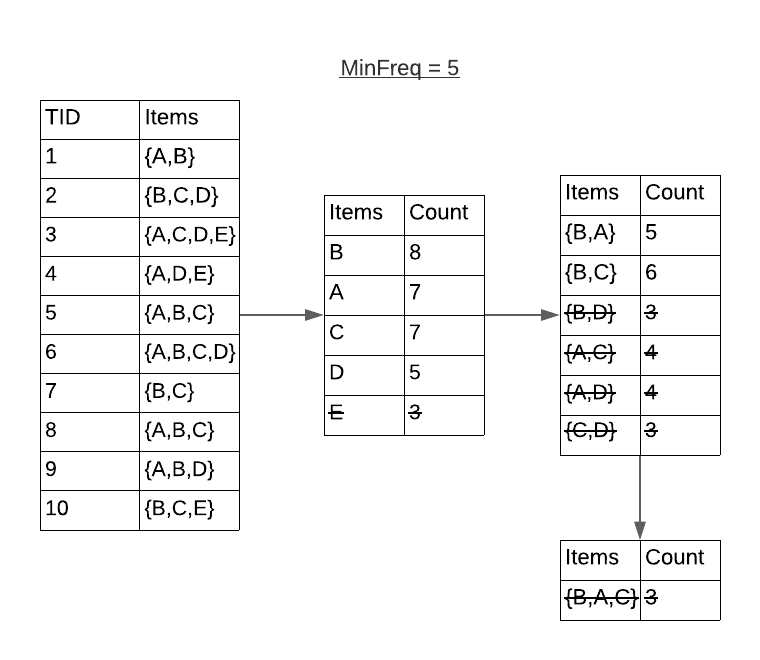
\includegraphics[width=\linewidth]{figures/aprioriexample}
  \caption{Apriori Example}
  \label{fig:aprioriexample}
\end{figure}

\begin{figure}
  \centering
  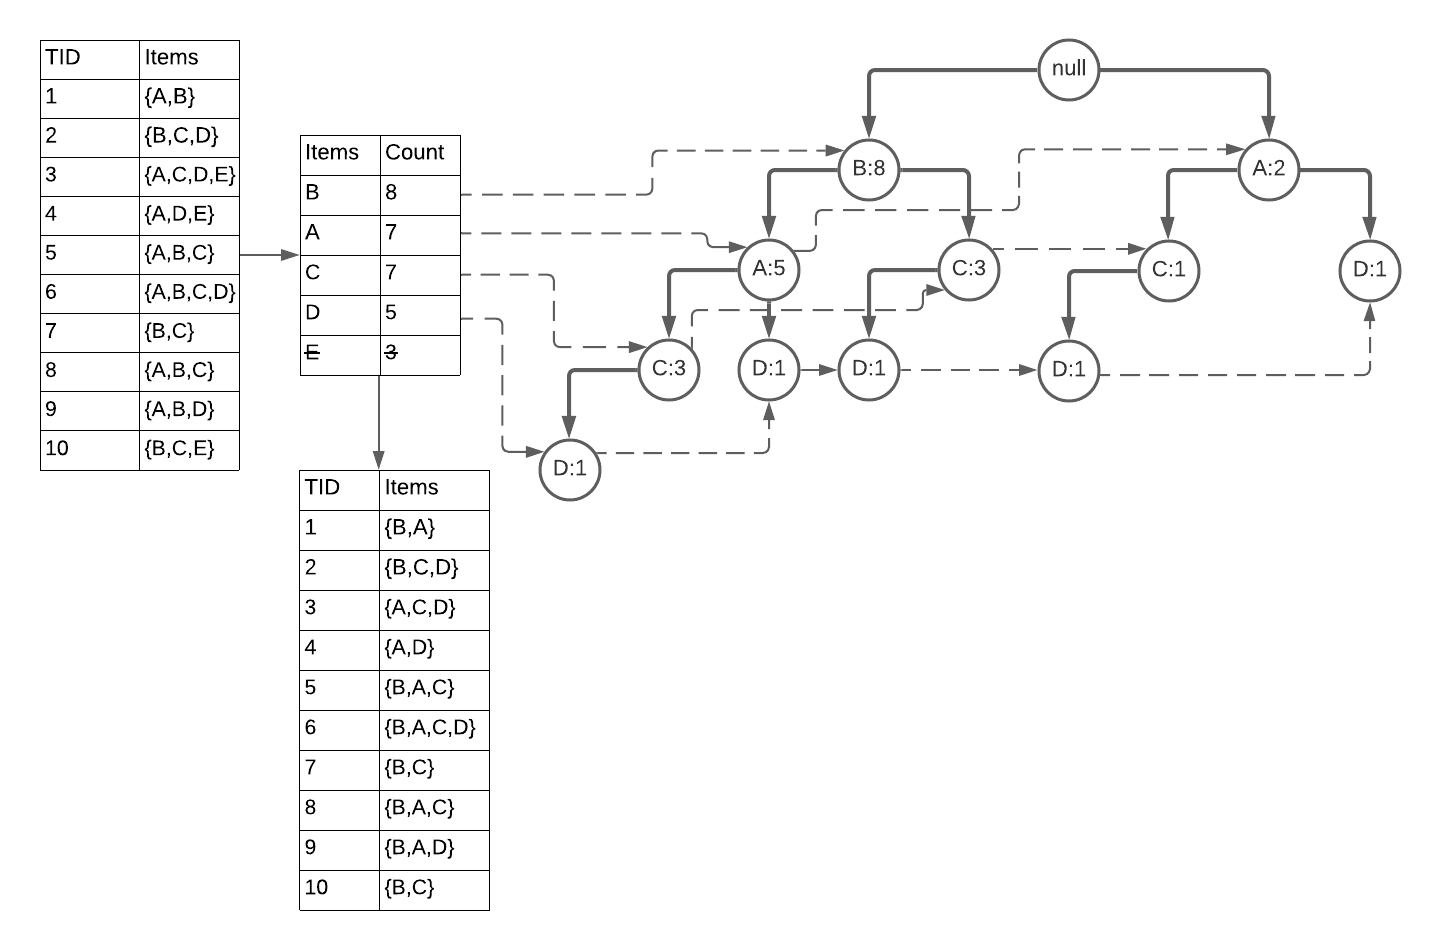
\includegraphics[width=\linewidth]{figures/FPTree}
  \caption{FPGrowth example}
  \label{fig:fpgrowthexample}
\end{figure}


It is important to mention that there might be some duplicates at several groups of frequent itemsets in stage 3.6, but this is solved when filtering the 1-length items that are not relevant to the specific group. This duplication also affects the size of the generated trees and overall memory.

\subsection{Incremental and Parallel Frequent itemsets mining}

Combining the previous 2 sections, yields an algorithm that does not rely on frequency order and uses parallelism advantages for computations of FIS.
The drawbacks are also drawn from the 2 algorithms - large memory consumption for saving all items and recursively calculating FIS. As we will show later in the \hyperref[sec:improvements]{Improvments} section, using an approach similar to ~\cite{kohefficient} and maintaining a pre-min support, together with using a semi-freq-order as in ~\cite{tanbeer2009efficient}, will significantly improve memory and mining runtime results.

\subsection{Song et al. }
A paper by Song et el.~\cite{song2017} proposes 2 techniques for building and mining frequent itemsets - IncBuildingPFP and IncMiningPFP. IncBuildingPFP presents a parallel model based on CanTree that supports incremental mining. The approach is presented in %TODO: add link
.  


\subsubsection{IncMiningPFP}
As discussed by Song et el.~\cite{song2017} (and analysed later in this article as well), using CanTree as is, will result in memory and time limitation for relatively medium datasets (>1M) even with large clusters (>100G RAM).  IncMiningPFP solves the problem of mining by constructing FP-Growth tree for shards with new incremental items. For other shards, the data is taken from cache.

IncMiningPFP consists of the following steps:
\begin{steps}
	\item Find global frequency list, F-List
	\item Group items G-list
	\item For the base case, for each shard, save the FIS and construct CanTrees to save all transactions.
	\item For every Shard:
			\begin{enumerate}
			\item find 1-size FIS, extract paths from CanTree that contain only those items and build a PF-Growth tree.
			\item Extract full FIS from FP-Growth tree and save items in shard cache.
			\end{enumerate}
	\item For every iteration dD, devide based on G-List and send to the appropriate shards.
	\item For every shard: 
				\begin{enumerate}
				\item If got new items from dD, update tree with new values
				\item If this shard has added transactions, recalculate new FIS in similar way to initial stage and update shard cache. 
				\item Return Caches FIS.
				\end{enumerate}
	\item Reduce all previous FIS, similar to PFP.
\end{steps}
